\section{Lyginamoji metodų analizė}\label{sec:experiments}

Lyginamosios analizės tikslas -- ištirti kenkėjiškų programų detektorių tikslumą \glsko{adversarial} sąlygomis. Lyginami originalus (nepakeistas) detektorius, autoriaus siūlomas \LIME ir \gls{mca} sintezės metodas \skyrius{sec:method} bei atskiros jo sudedamosios dalys: \LIME metodo pritaikymas \gls{ae} aptikimui \skyrius{sec:literature:defense:ids} ir \gls{mca} transformacijos klasifikatorius \skyrius{sec:literature:dimensions:mca}.

% Describe how the experiments are performed

\subsection{Tyrimo metodika}

Visa tyrimo metodika pavaizduota \ref{fig:methodology}-ame pav. Tyrimui pasirinktas \SLEIPNIR \cite{al-dujailiAdversarialDeepLearning2018} duomenų rinkinys, kuriame yra $34995$ kenkėjiškų programų ir $19696$ nekenkėjiškų programų pavyzdžių, užkoduotų $22761$-mačiais dvejetainiais vektoriais. Iš šio rinkinio pasirinkta po $1500$ unikalių kenkėjiškų ir nekenkėjiškų programų pavyzdžių paliekant pirmas $200$ komponenčių -- taip gaunamas subalansuotas duomenų rinkinys. Šis rinkinys toliau skeliamas į mokymo ir testavimo aibes santykiu $4:1$.
Eksperimentams atlikti paruošiamos šios priemonės:
\begin{enumerate}
    \item Testavimo duomenų aibė, iš kurios sudaromas trijų tipų programų požymių srautas: nekenkėjiškos, kenkėjiškos, kenkėjiškos-obfuskuotos.
    \item \textit{MalGAN} \cite{huGeneratingAdversarialMalware2017} \gls{ae} generatorius. Pasirinkimo motyvacija pateikiama \ref{sec:method:malgan} poskyryje.
    \item Kenkėjiškų programų detektorius (klasifikatorius).
    \item \Glsplko{adversarial} aptikimo komponentas
    \begin{itemize}
        \item Naudojantis originalius požymius.
        \item Naudojantis \gls{mca} transformuotus požymius \skyrius{sec:method}.
    \end{itemize}
\end{enumerate}

\noindent
Su šiais įrankiais atliekami 4 eksperimentai \textbf{aplinkoje su \glsplkuo{adversarial}}:
    \begin{enumerate}
        \item Bazinis atvejis -- originalaus klasifikatoriaus tikslumo nustatymas.
        \item Klasifikatoriaus, naudojančio \gls{mca} transformuotus požymius, tikslumo nustatymas.
        \item Klasifikatoriaus praplėtimo su modifikuoto \LIME metodo pritaikymu \glsplko{adversarial} aptikimui tikslumo nustatymas.
        \item Klasifikatoriaus praplėtimo su \LIME ir \gls{mca} metodų sinteze \glsplko{adversarial} aptikimui tikslumo nustatymas.
    \end{enumerate}

\begin{figure}[h]
    \centering
    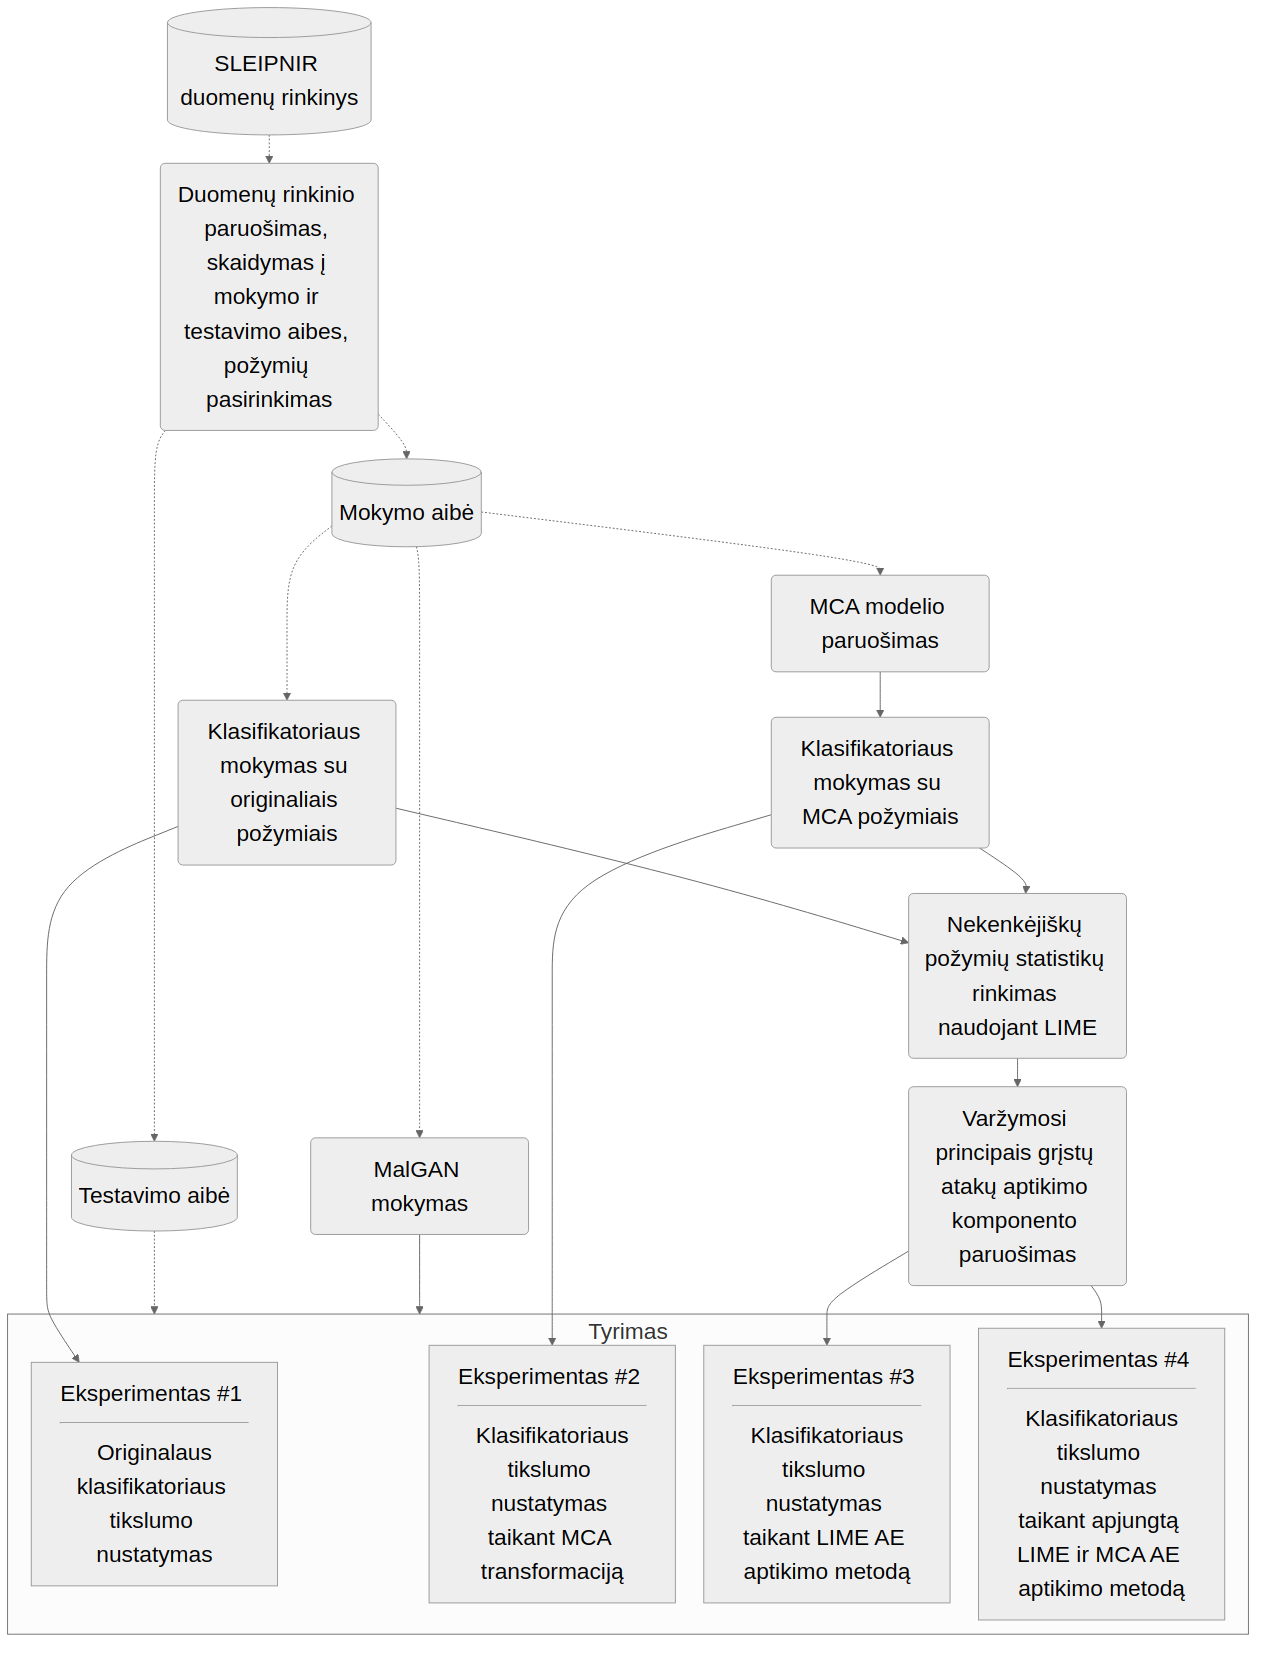
\includegraphics[width=\textwidth]{images/methodology.png}
    \caption{Tyrimo metodika}
    \label{fig:methodology}
\end{figure}

\subsection{\Glsplko{adversarial} \glsko{framework} pasirinkimas}\label{sec:method:malgan}

Tyrimui pasirinktas \refFramework{MalGAN} \gls{framework} dėl šių priežasčių:
\begin{itemize}
    \item \gls{gan} yra vieni iš perspektyviausių ir efektyviausių \gls{ml} modelių \gls{ae} generavimui.
    \item \textit{MalGAN} yra plačiai naudojamas kaip bazinis modelis tolimesniems tyrimas, yra kelios atviro kodo repozitorijos\footnote{Šiam tyrimui pasirinkta https://github.com/ZaydH/MalwareGAN repozitorija, kaip pradinis \textit{MalGAN} įgyvendinimas}, įgyvendinančios šį \glska{framework}.
    \item \textit{MalGAN} naudoja dvejetainius požymių vektorius. Būtent tokie požymiai turėtų kelti sunkumų esamiems \gls{ae} aptikimo metodams \skyrius{sec:method:mods}.
\end{itemize}

\clearpage
\subsection{\gls{mca} komponenčių pasirinkimas}\label{sec:method:mca_comp_selection}
Komponenčių pasirinkimas yra \ref{fig:methodology}-ame pav. minimo \gls{mca} modelio paruošimo dalis. Komponenčių pasirinkimui \ty jų kiekio pasirinkimui nėra apibrėžto \enquote{teisingo} metodo \cite{abdiPrincipalComponentAnalysis2010}. Dažniausiai siūlomi metodai yra tik didesnių už $1$ tikrinių reikšmių pasirinkimas ir \textit{alkūnės} \angl{scree / elbow} metodas. Šie metodai netiko, nes juos taikant paliktos \gls{mca} komponentės nepaaiškintų net pusės visos \glsko{inertia}: visos tikrinės reikšmės analizuojamuose mokymo duomenyse yra $<1$, o alkūnės taške sukaupta \gls{inertia} yra $\num{47,62} \%$ \zr{fig:inertia}. Taigi, pasirinkti 2 nestandartiniai \gls{mca} komponenčių kiekio kriterijai: 

\noindent
\begin{minipage}[l]{0.48\textwidth}
    \vspace{-2cm}
    \begin{itemize}[leftmargin=*]
        \item sukaupta \gls{inertia} $\ge 75\%$,
        \item išmokyto klasifikatoriaus tikslumas $\hat{a}$ nemažesnis nei originalaus klasifikatoriaus tikslumas $a$ $5\%$ intervale ($\hat{a} \ge a - 5\%$), kai įvesčių srautas normalus (nėra obfuskuotų programų požymių -- \gls{ae}). Šiuo atveju $\hat{a} \ge \num{\mathOp{\accNoAttackNormal - 0.05}}$ \Zr{tbl:safe:original:metrics}
    \end{itemize}
\end{minipage}
\hspace{0.02\textwidth}
\begin{minipage}{0.5\textwidth}
    \centering
    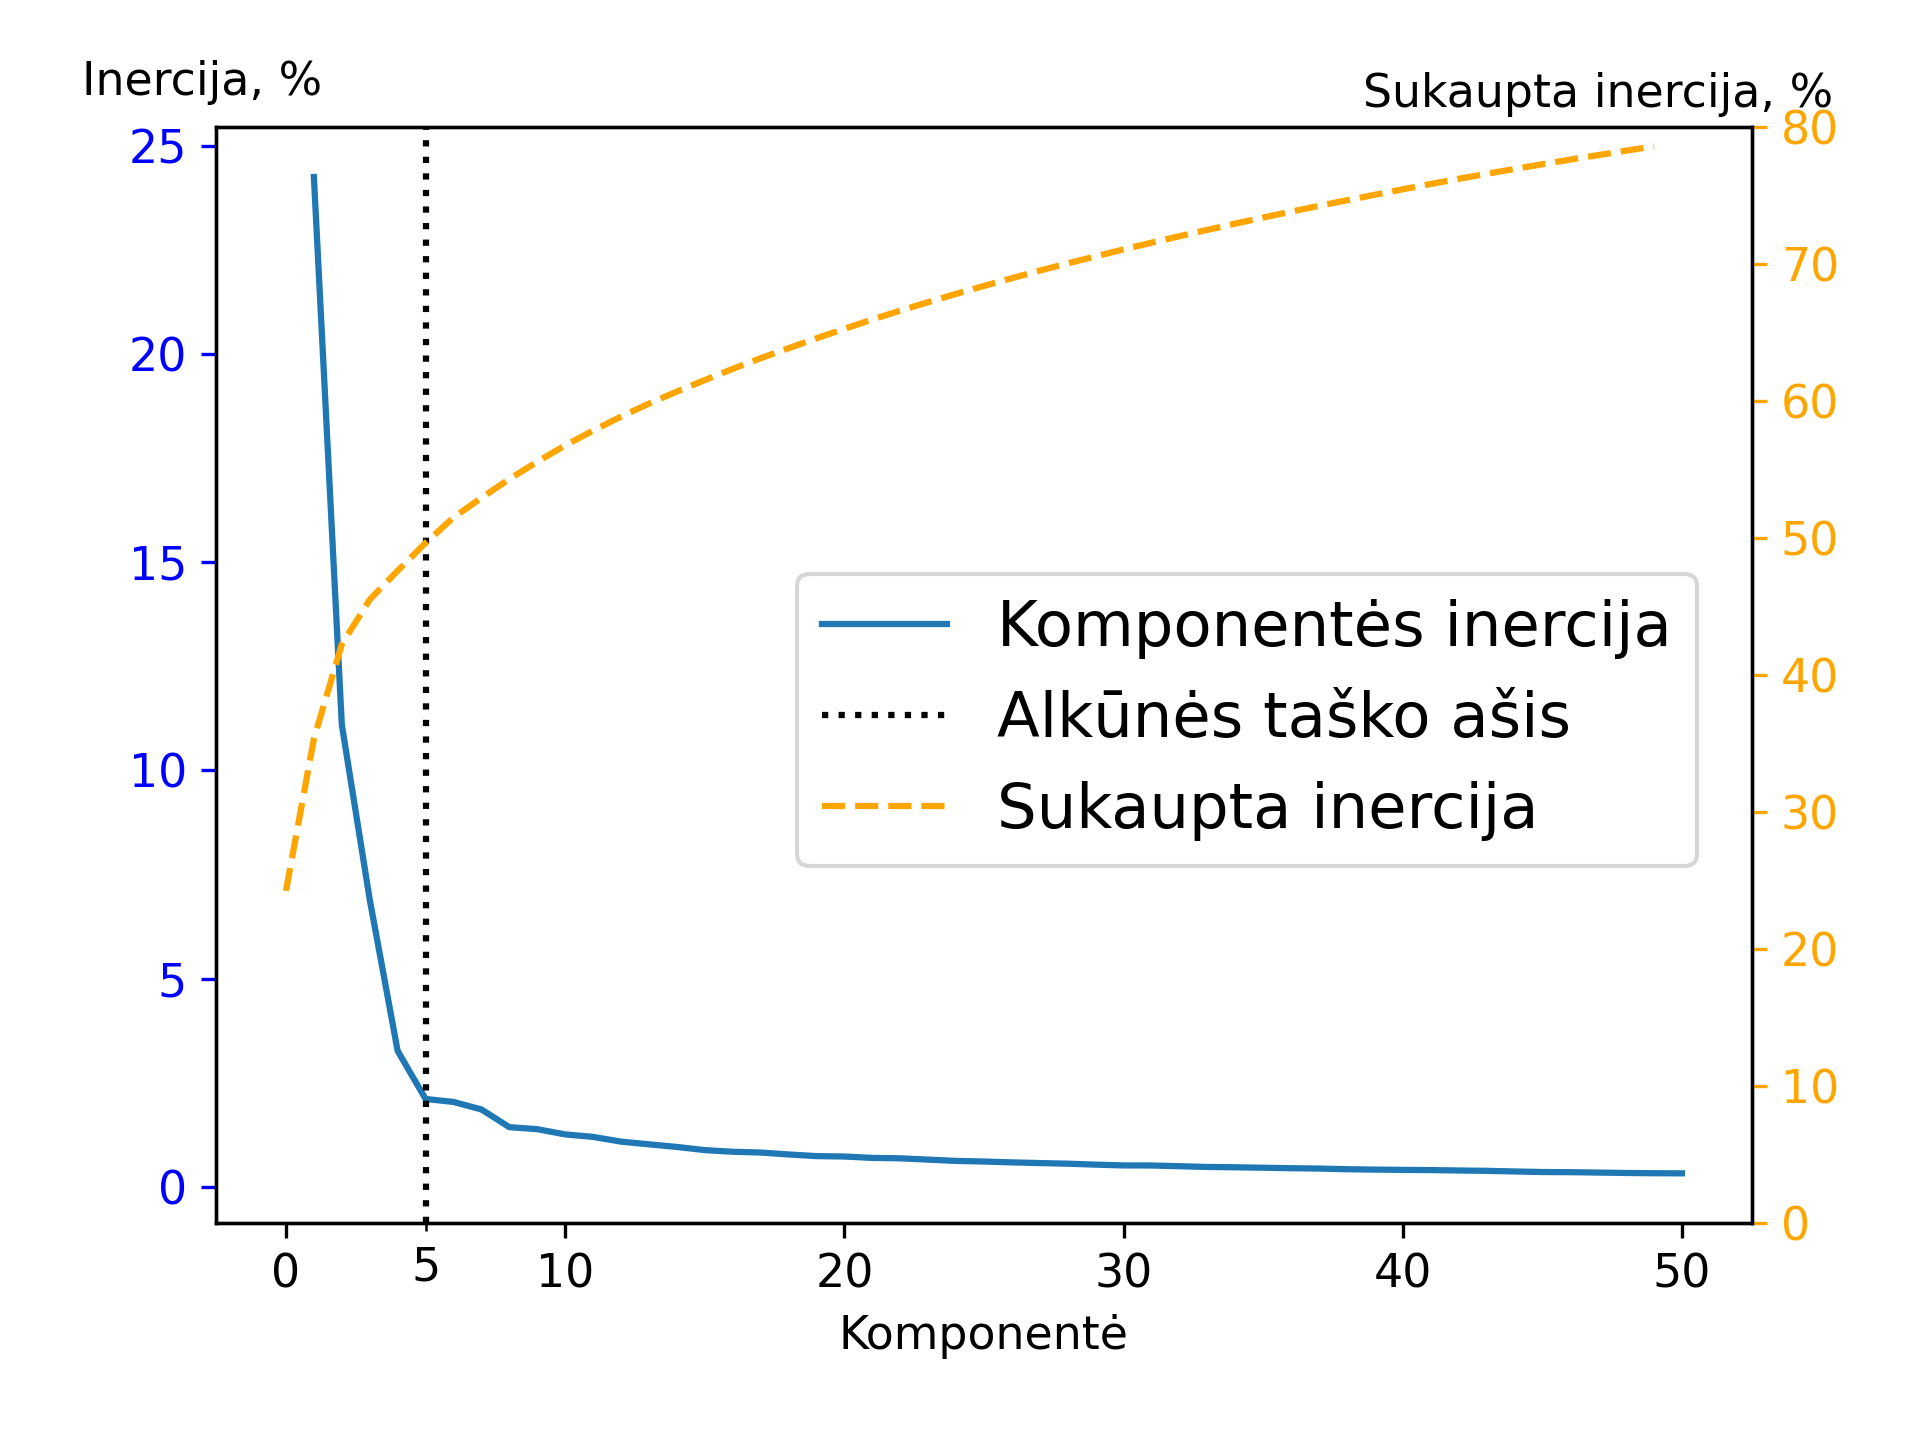
\includegraphics[width=\textwidth]{images/scree.png}
    \vspace{-1cm}
    \captionof{figure}{\textit{Alkūnės} analizė \gls{mca} inercijai}
    \label{fig:inertia}
\end{minipage}

\begin{table}[h]
    \centering
    \caption{Originalaus klasifikatoriaus metrikos, kai nevykdoma \gls{adversarial}}
    \exptable[\accNoAttackNormal]{tables/original_no_attack.csv}
    \label{tbl:safe:original:metrics}
\end{table}
\begin{table}[h]
    \centering
    \caption{\gls{mca} klasifikatoriaus metrikos, kai nevykdoma \gls{adversarial}}
    \exptable[\accNoAttackMca]{tables/mca_no_attack.csv}
    \label{tbl:safe:mca:metrics}
\end{table}

\def\accumulatedInertia{$78,57\%$}

\ref{tbl:safe:mca:metrics}-oje lentelėje pavaizduotos \gls{mca} transformacijos klasifikatoriaus metrikos gaunamos pasirinkus 50 komponenčių (suspaudimo santykis $4:1$), kurių sukaupta \gls{inertia} yra \accumulatedInertia. Kadangi \accumulatedInertia $\;> 75\%$ ir $\num{\accNoAttackMca} > \num{\mathOp{\accNoAttackNormal - 0.05}}$, abu \gls{mca} komponenčių kiekio kriterijai yra tenkinami.

% --- PCA/MCA
% Show graphs of 2 best components (~30% of inertia)
% Show knee analysis of 50 then 9 components

\clearpage
\subsection{Eksperimentai}
\subsubsection{Originalaus klasifikatoriaus tikslumo nustatymas}% Show graphs and classification results when hit with obfuscation

Kaip ir tolimesniuose eksperimentuose, testavimo duomenų aibė šiam
eksperimentui susideda iš 300 kenkėjiškų ir 300 nekenkėjiškų programų požymių.
Taip pat pridedami dar 300 obfuskuotų programų požymių (jie gaunami naudojant
jau turimus kenkėjiškų programų požymius ir išmokytą \MALGAN modelį).

Kadangi originalus klasifikatorius negali diferencijuoti obfuskuotų programų,
turima duomenų aibė nėra subalansuota -- turime dvigubai daugiau duomenų,
kuriuos klasifikatorius turėtų klasifikuoti kaip kenkėjiškus. Dėl to,
klasifikacijos lentelėje \zr{fig:exp1:confusion} rodomas prognozuojamos klasės
ir visų tai klasei priklausančių duomenų santykis (tokios matricos pagrindinė
diagonalė nurodo klasės atkūrimo statistiką \angl{recall}).

Eksperimento rezultatai (klasifikavimo metrikos) pateikiami \ref{tbl:exp1:metrics}-oje lentelėje.
\begin{figure}[h]
    \centering
    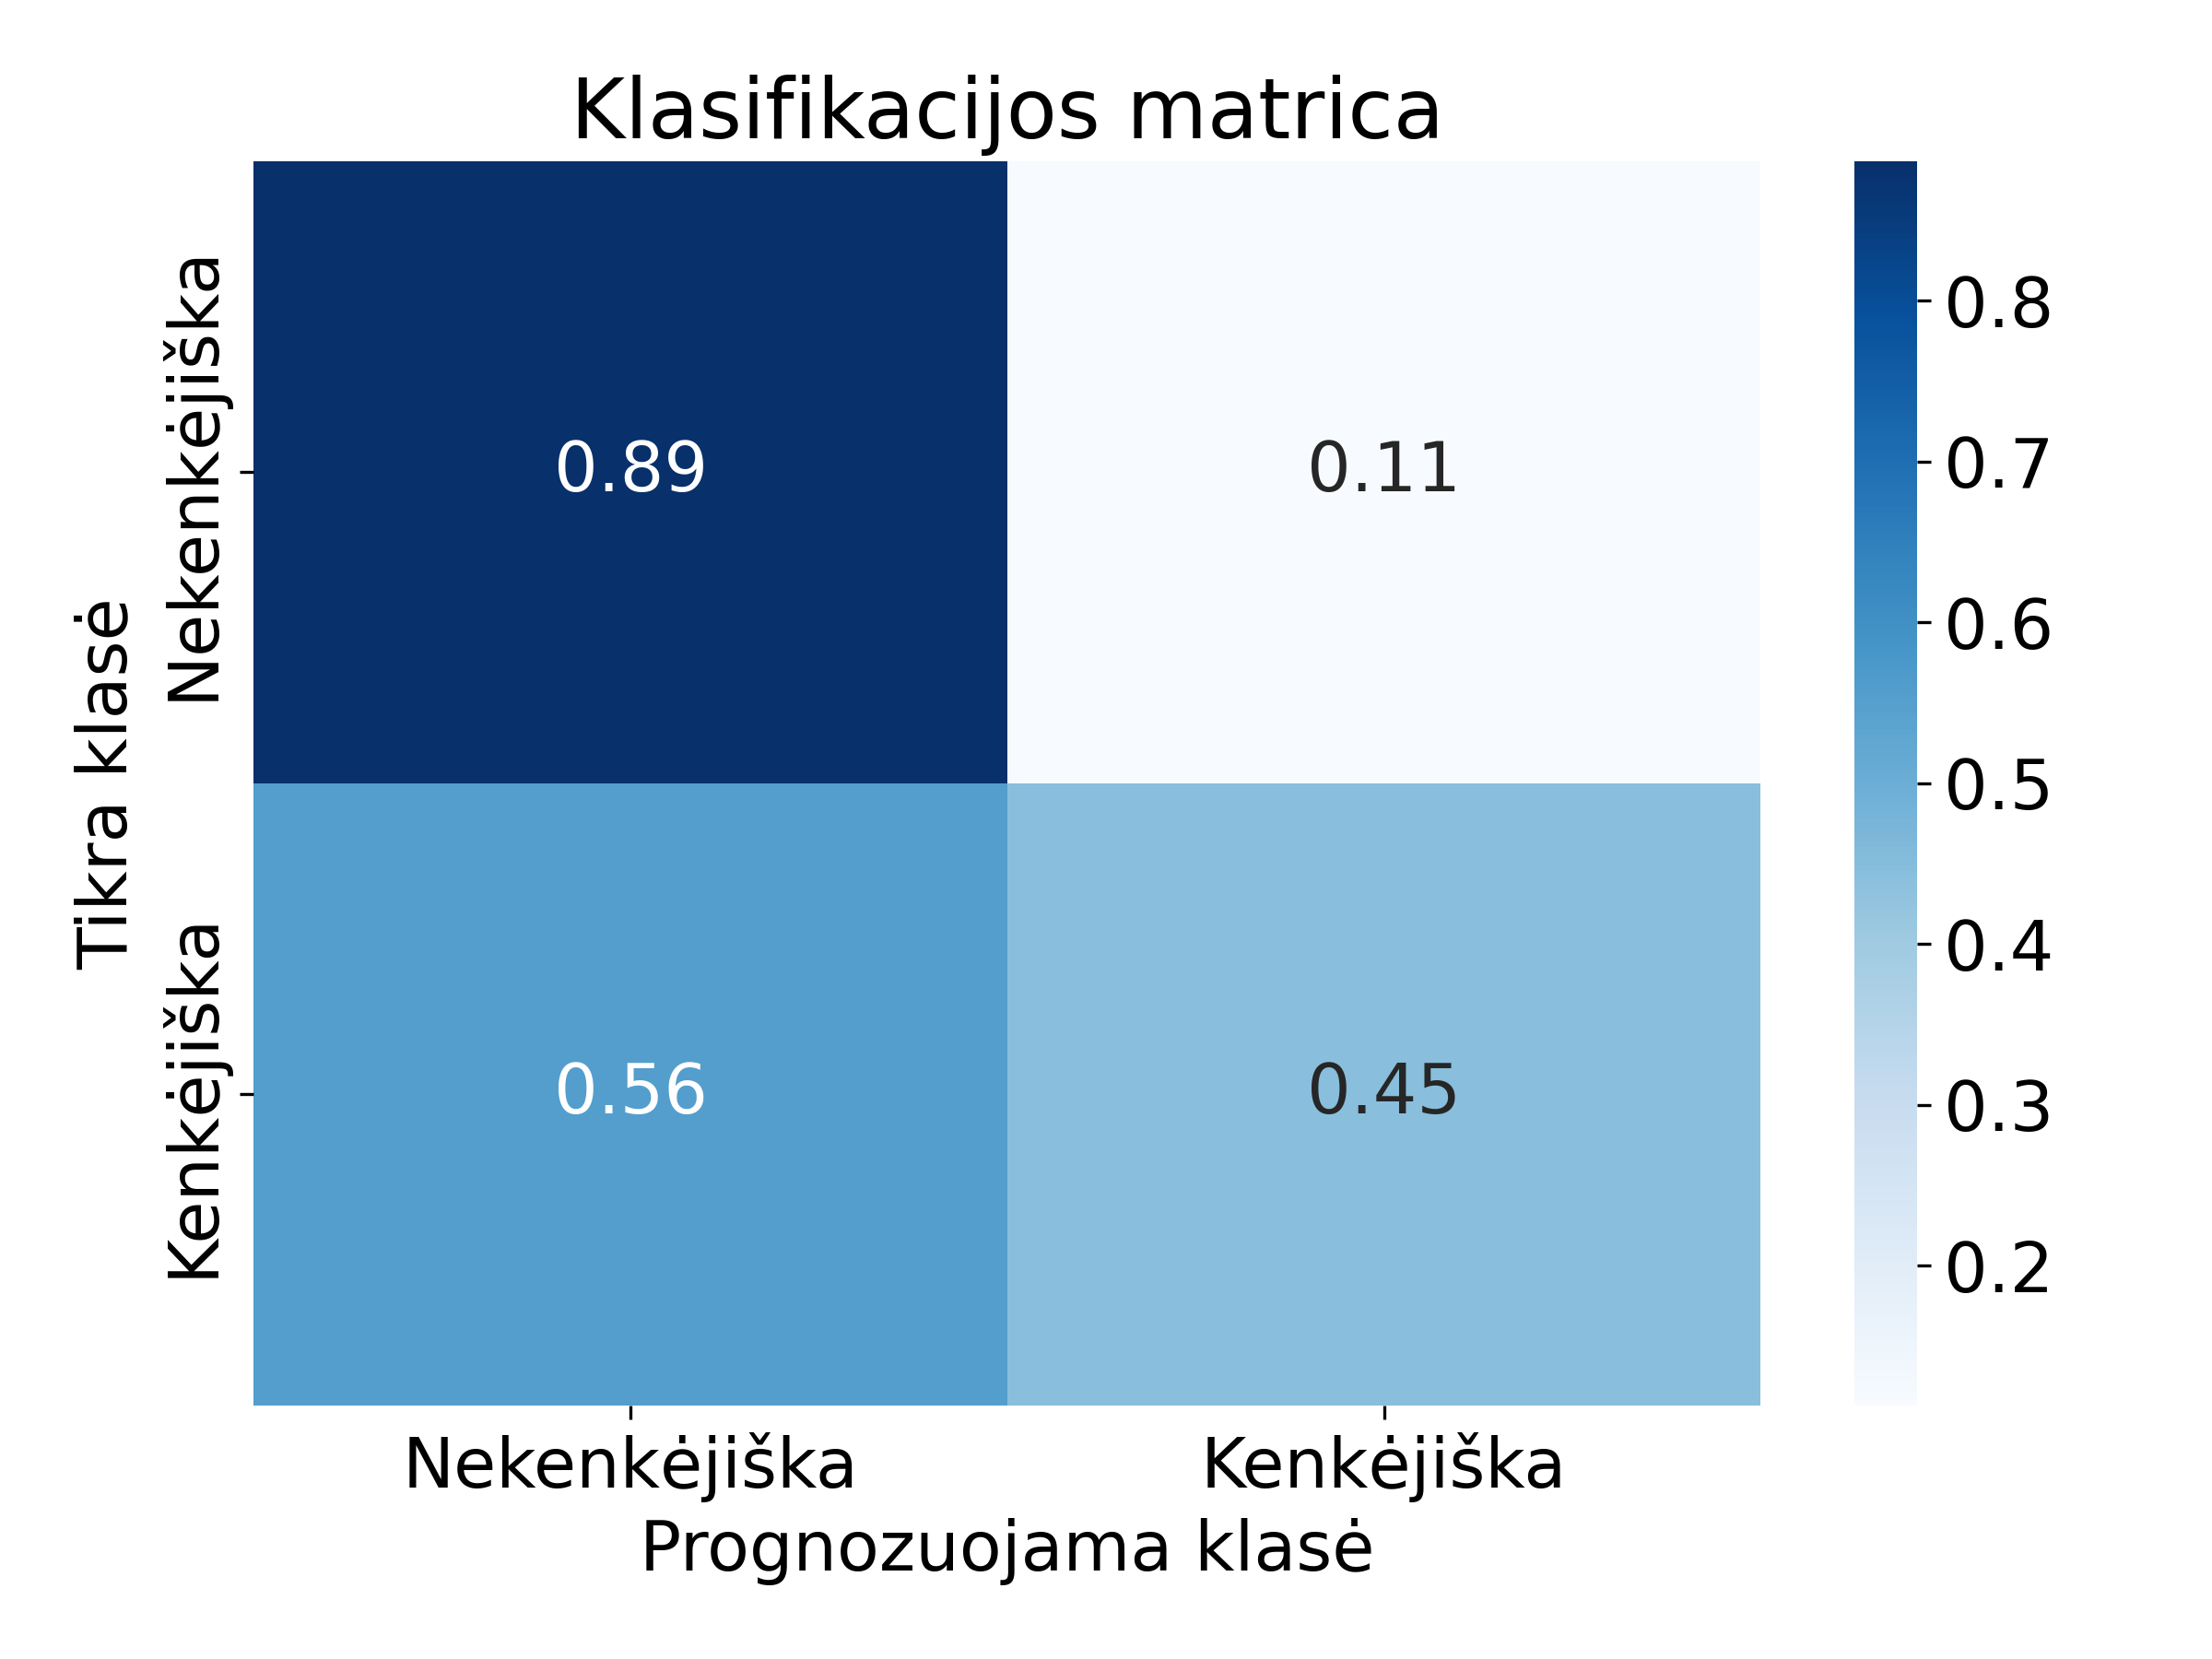
\includegraphics[width=0.45\textwidth]{images/normal_2x2.png}
    \caption{Klasifikavimo matrica}
    \label{fig:exp1:confusion}
\end{figure}

\begin{table}[h]
    \caption{Originalaus klasifikatoriaus metrikos}
    \centering
    \exptable[\accNormal]{tables/normal_2x2.csv}
    \label{tbl:exp1:metrics}
\end{table}
\clearpage
\subsubsection{\gls{mca} transformacijos klasifikatoriaus tikslumo nustatymas}\label{sec:exp:4}

\gls{mca} klasifikatorius yra vienas iš standartinių klasifikatorių (šiuo atveju atsitiktinio miško \angl{random forest}), naudojantis pakeistos bazės požymius kaip įvestį. Šioje vietoje naudojamas klasifikatorius gali būti bet koks, tačiau turi būti suderinamas su \gls{mca} komponenčių kiekio reikalavimais \skyrius{sec:method:mca_comp_selection}. 

Kaip ir originalus klasifikatorius, šis negeba išskirti obfuskuotų programų, tad \ref{fig:exp4:confusion} pav. pateikiamoje klasifikavimo lentelėje rodomas prognozuojamos klasės ir visų tai klasei priklausančių duomenų santykis.
Eksperimento rezultatai (klasifikavimo metrikos) pateikiami \ref{tbl:exp4:metrics}-oje lentelėje.
\begin{figure}[h]
    \centering
    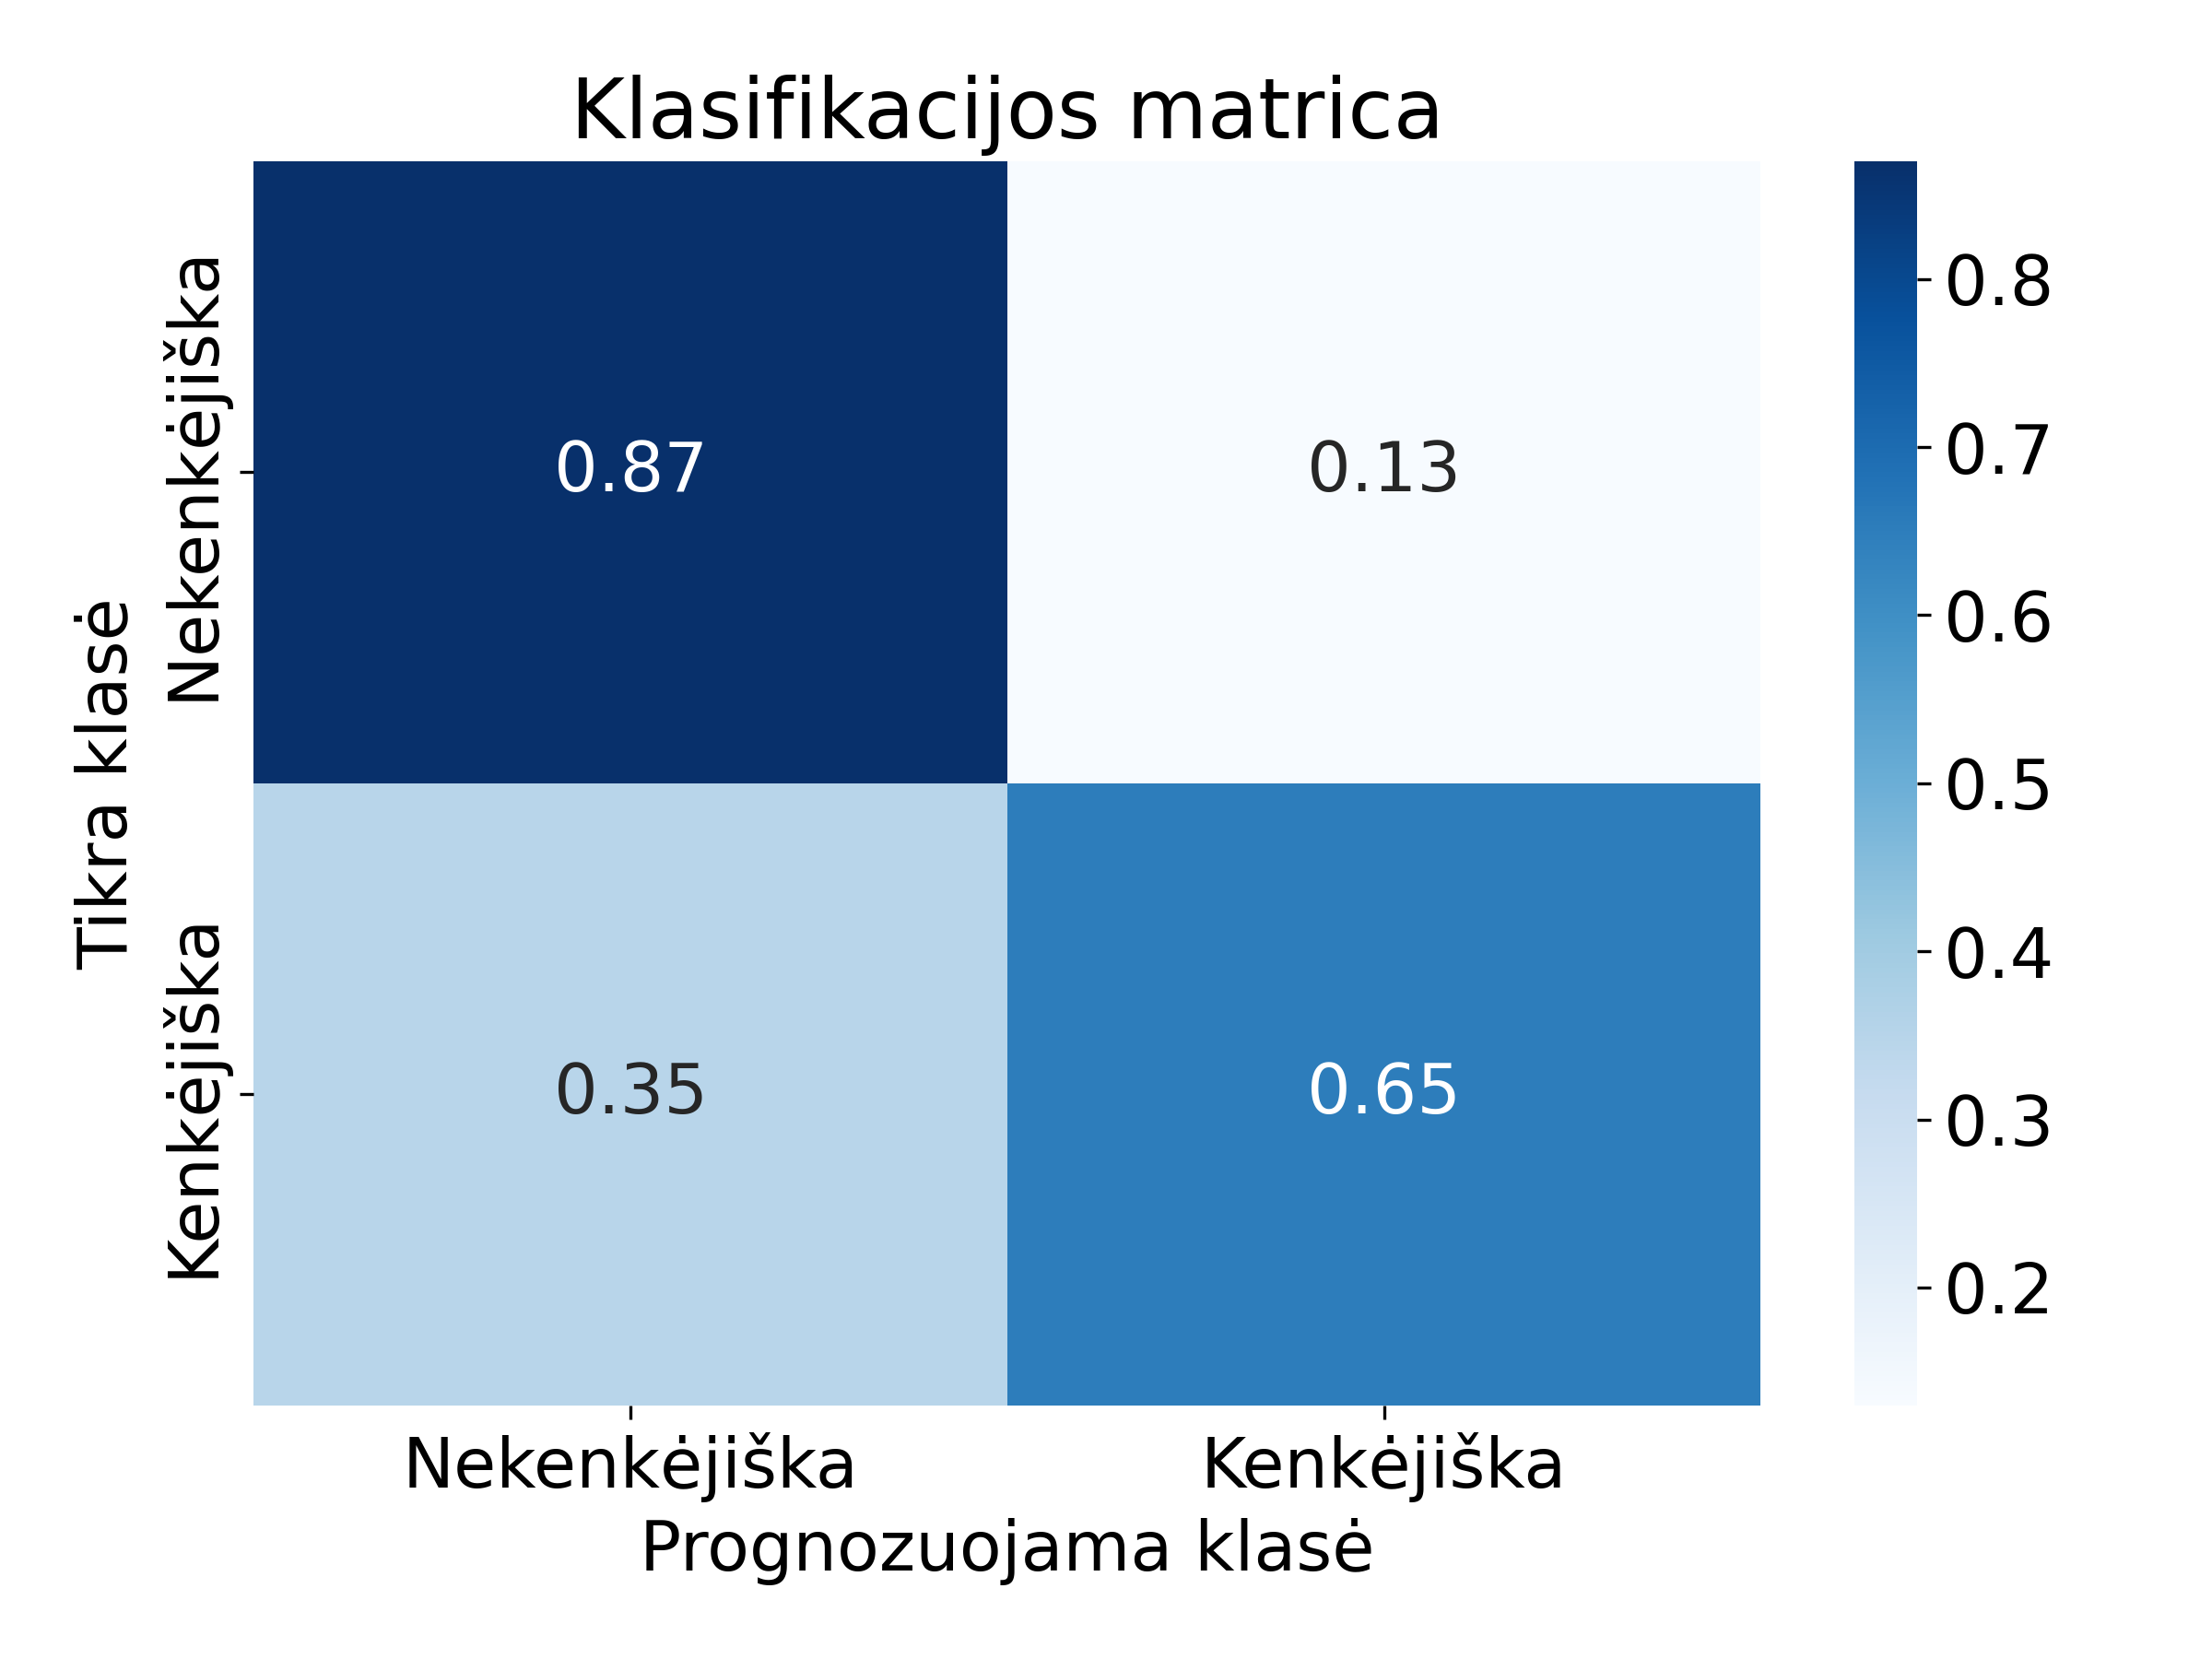
\includegraphics[width=0.5\textwidth]{images/mca_2x2.png}
    \caption{Klasifikavimo matrica}
    \label{fig:exp4:confusion}
\end{figure}

\begin{table}[h]
    \caption{\gls{mca} transformacijos klasifikatoriaus metrikos}
    \centering
    \exptable[\accMcaEquiv]{tables/mca_2x2.csv}
    \label{tbl:exp4:metrics}
\end{table}
\clearpage
\subsubsection{Modifikuoto \LIME pritaikymo \gls{ae} aptikimui tikslumo nustatymas}\label{sec:exp:2}

Šio eksperimento tikslas yra nustatyti modifikuoto \LIME pritaikymo \gls{ae} aptikimui \poskyris{sec:method:mods} tikslumą. \LIME branduolio plotis paliekamas pagal numatytus nustatymus ($\omega = 0,75 \cdot \sqrt{n}$, čia $n$ -- požymių skaičius, taigi, $\omega = 0,75 \cdot \sqrt{200} \approx 10,61$) \cite{ribeiroWhyShouldTrust2016}.

Kadangi šis metodas geba aptikti \gls{ae} -- obfuskuotas programas --
\ref{fig:exp2:confusion} pav. pateikiamos dvi klasifikacijos lentelės. Pirmoje (\ref{fig:exp2:confusion:a}) -- klasifikacijos rezultatai, kai obfuskuota programa laikoma kenkėjiška. Antroje (\ref{fig:exp2:confusion:b}) -- išskiriama \textit{obfuskuota} klasė. Kadangi išskyrus šią klasę duomenų rinkinys tampa subalansuotas, klasifikavimo lentelėje pateikiami sveiki skaičiai, atitinkantys modelio prognozuojamų duomenų tai klasei kiekį.

Eksperimento rezultatai (klasifikavimo metrikos) pateikiami \ref{tbl:exp2:metrics2}-oje ir \ref{tbl:exp2:metrics3}-oje lentelėse.
\begin{figure}[h]
    \begin{subfigure}{0.5\textwidth}
        \centering
        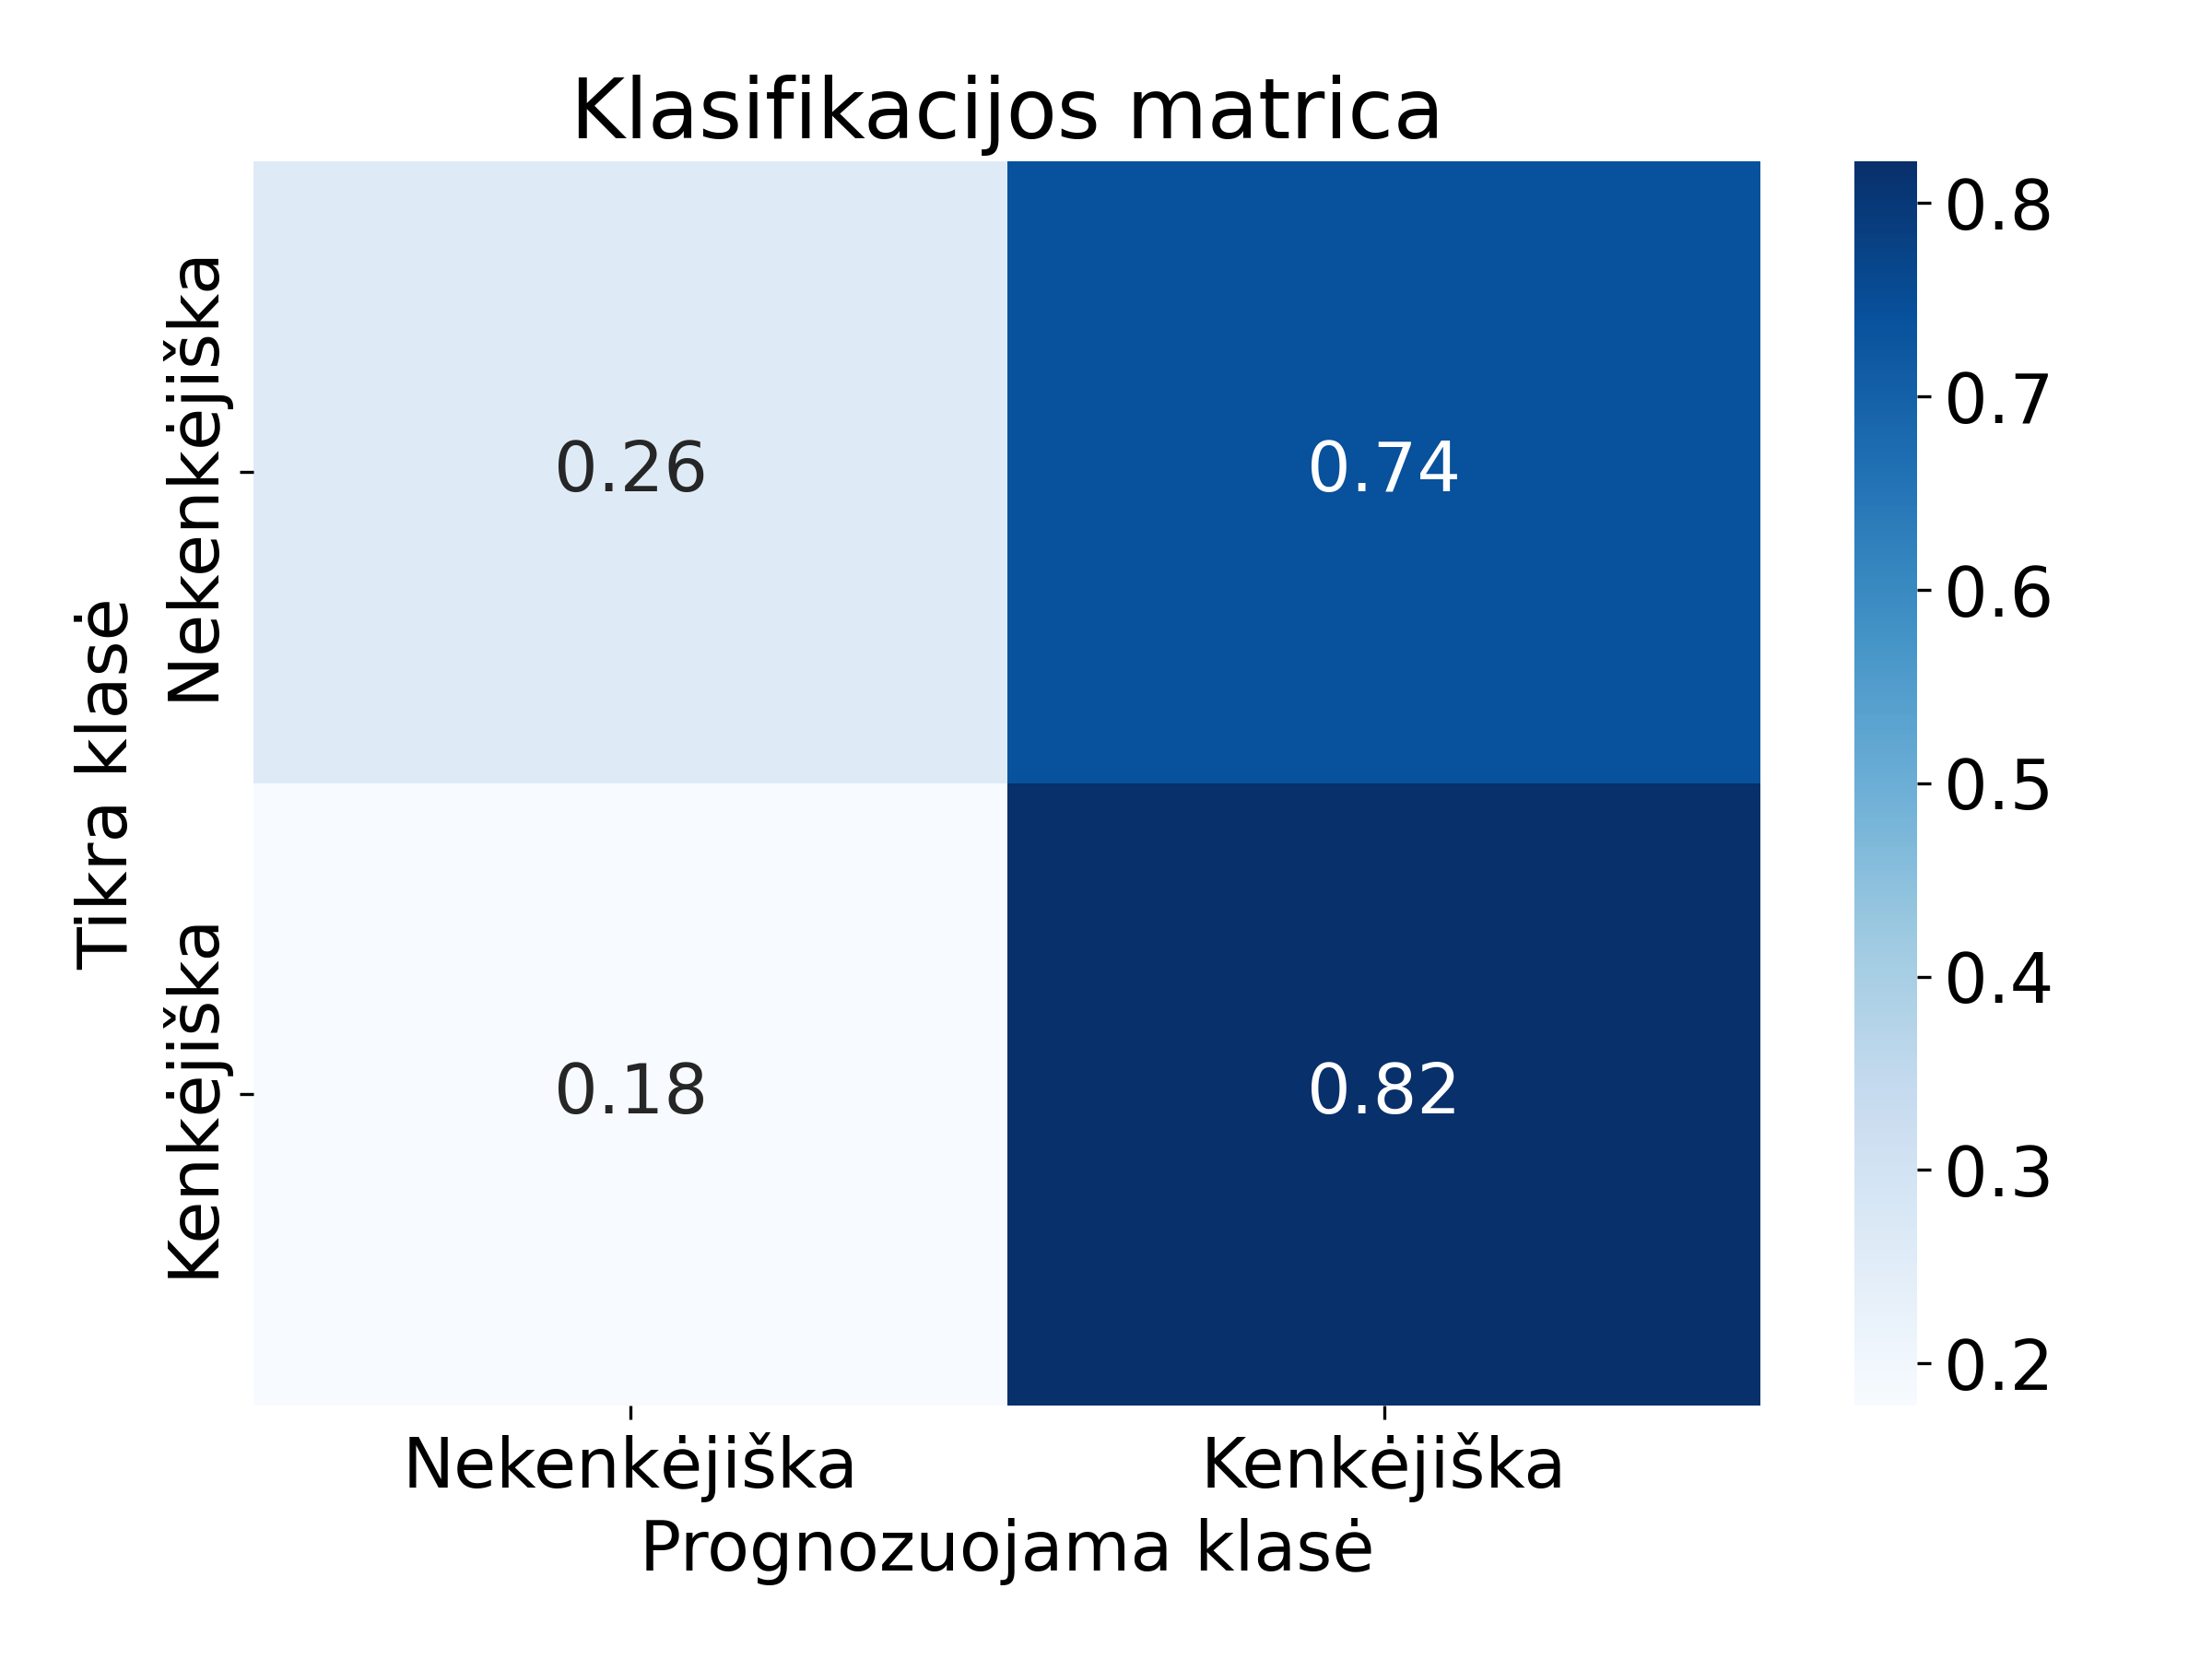
\includegraphics[width=\textwidth]{images/lime_2x2.png}
        \caption{Neišskiriant \textit{obfuskuotų} pavyzdžių klasės}
        \label{fig:exp2:confusion:a}
    \end{subfigure}
    \begin{subfigure}{0.5\textwidth}
        \centering
        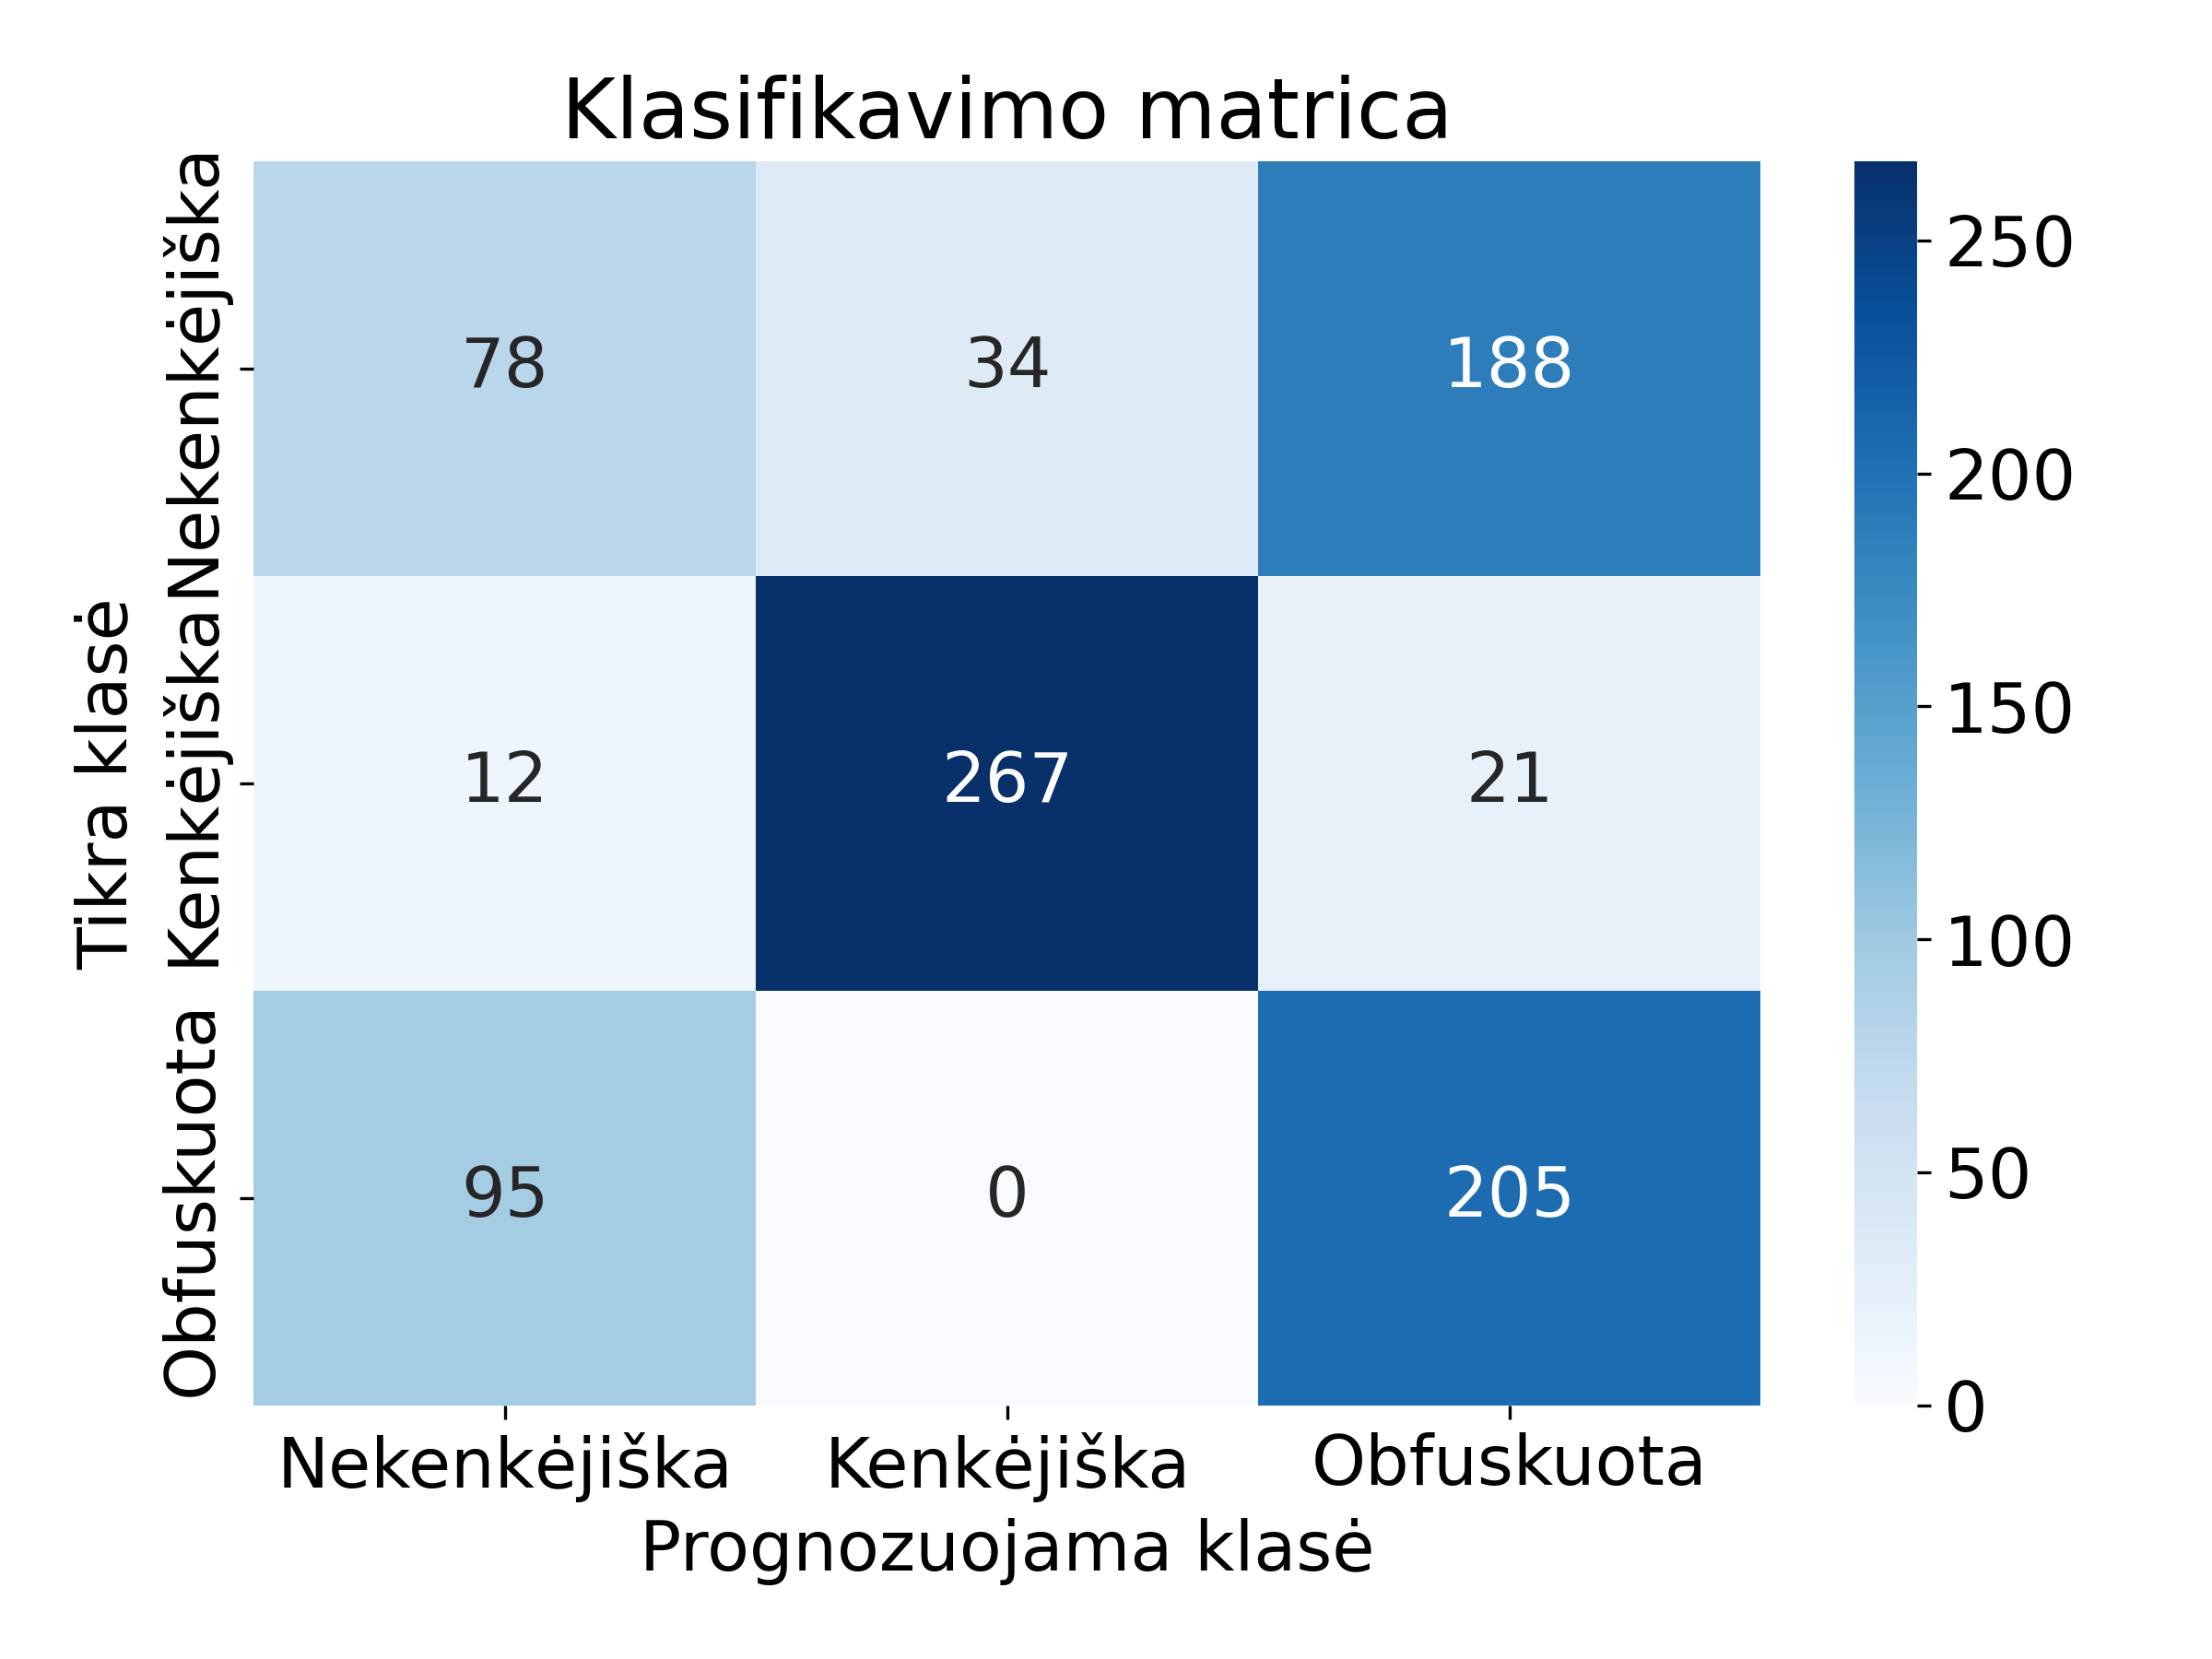
\includegraphics[width=\textwidth]{images/lime_3x3.png}
        \caption{Išskiriant \textit{obfuskuotų} pavyzdžių klasę}
        \label{fig:exp2:confusion:b}
    \end{subfigure}
    \caption{\LIME pritaikymo \gls{ae} aptikimui klasifikavimo lentelės}
    \label{fig:exp2:confusion}
\end{figure}

\begin{table}[h]
    \caption{\LIME pritaikymo \gls{ae} aptikimui klasifikatoriaus metrikos (neišskiriant \textit{obfuskuotos} klasės)}
    \centering
    \exptable[\accLimeCat]{tables/lime_2x2.csv}
    \label{tbl:exp2:metrics2}
\end{table}

\begin{table}[h]
    \caption{\LIME pritaikymo \gls{ae} aptikimui klasifikatoriaus metrikos (išskiriant \textit{obfuskuotą} klasę)}
    \centering
    \exptable[\accLimeCatObf]{tables/lime_3x3.csv}
    \label{tbl:exp2:metrics3}
\end{table}

% Use the paper method and show results that do not perform well
\clearpage
\subsubsection{\LIME ir \gls{mca} metodų sintezės tikslumo nustatymas}\label{sec:exp:3}

Šio eksperimento tikslas yra nustatyti autoriaus siūlomos modifikuoto \LIME ir \gls{mca} metodų sintezės \glsplko{adversarial} aptikimui tikslumą. Kaip ir praeitame eksperimente, \ref{fig:exp3:confusion}-ame pav. pateikiamos dvi klasifikavimo lentelės -- išskiriant ir neišskiriant \textit{obfuskuotą} klasę. 

Eksperimento rezultatai (klasifikavimo metrikos) pateikiami \ref{tbl:exp3:metrics2}-oje ir \ref{tbl:exp3:metrics3}-oje lentelėse.

\begin{figure}[h]
    \begin{subfigure}{0.5\textwidth}
        \centering
        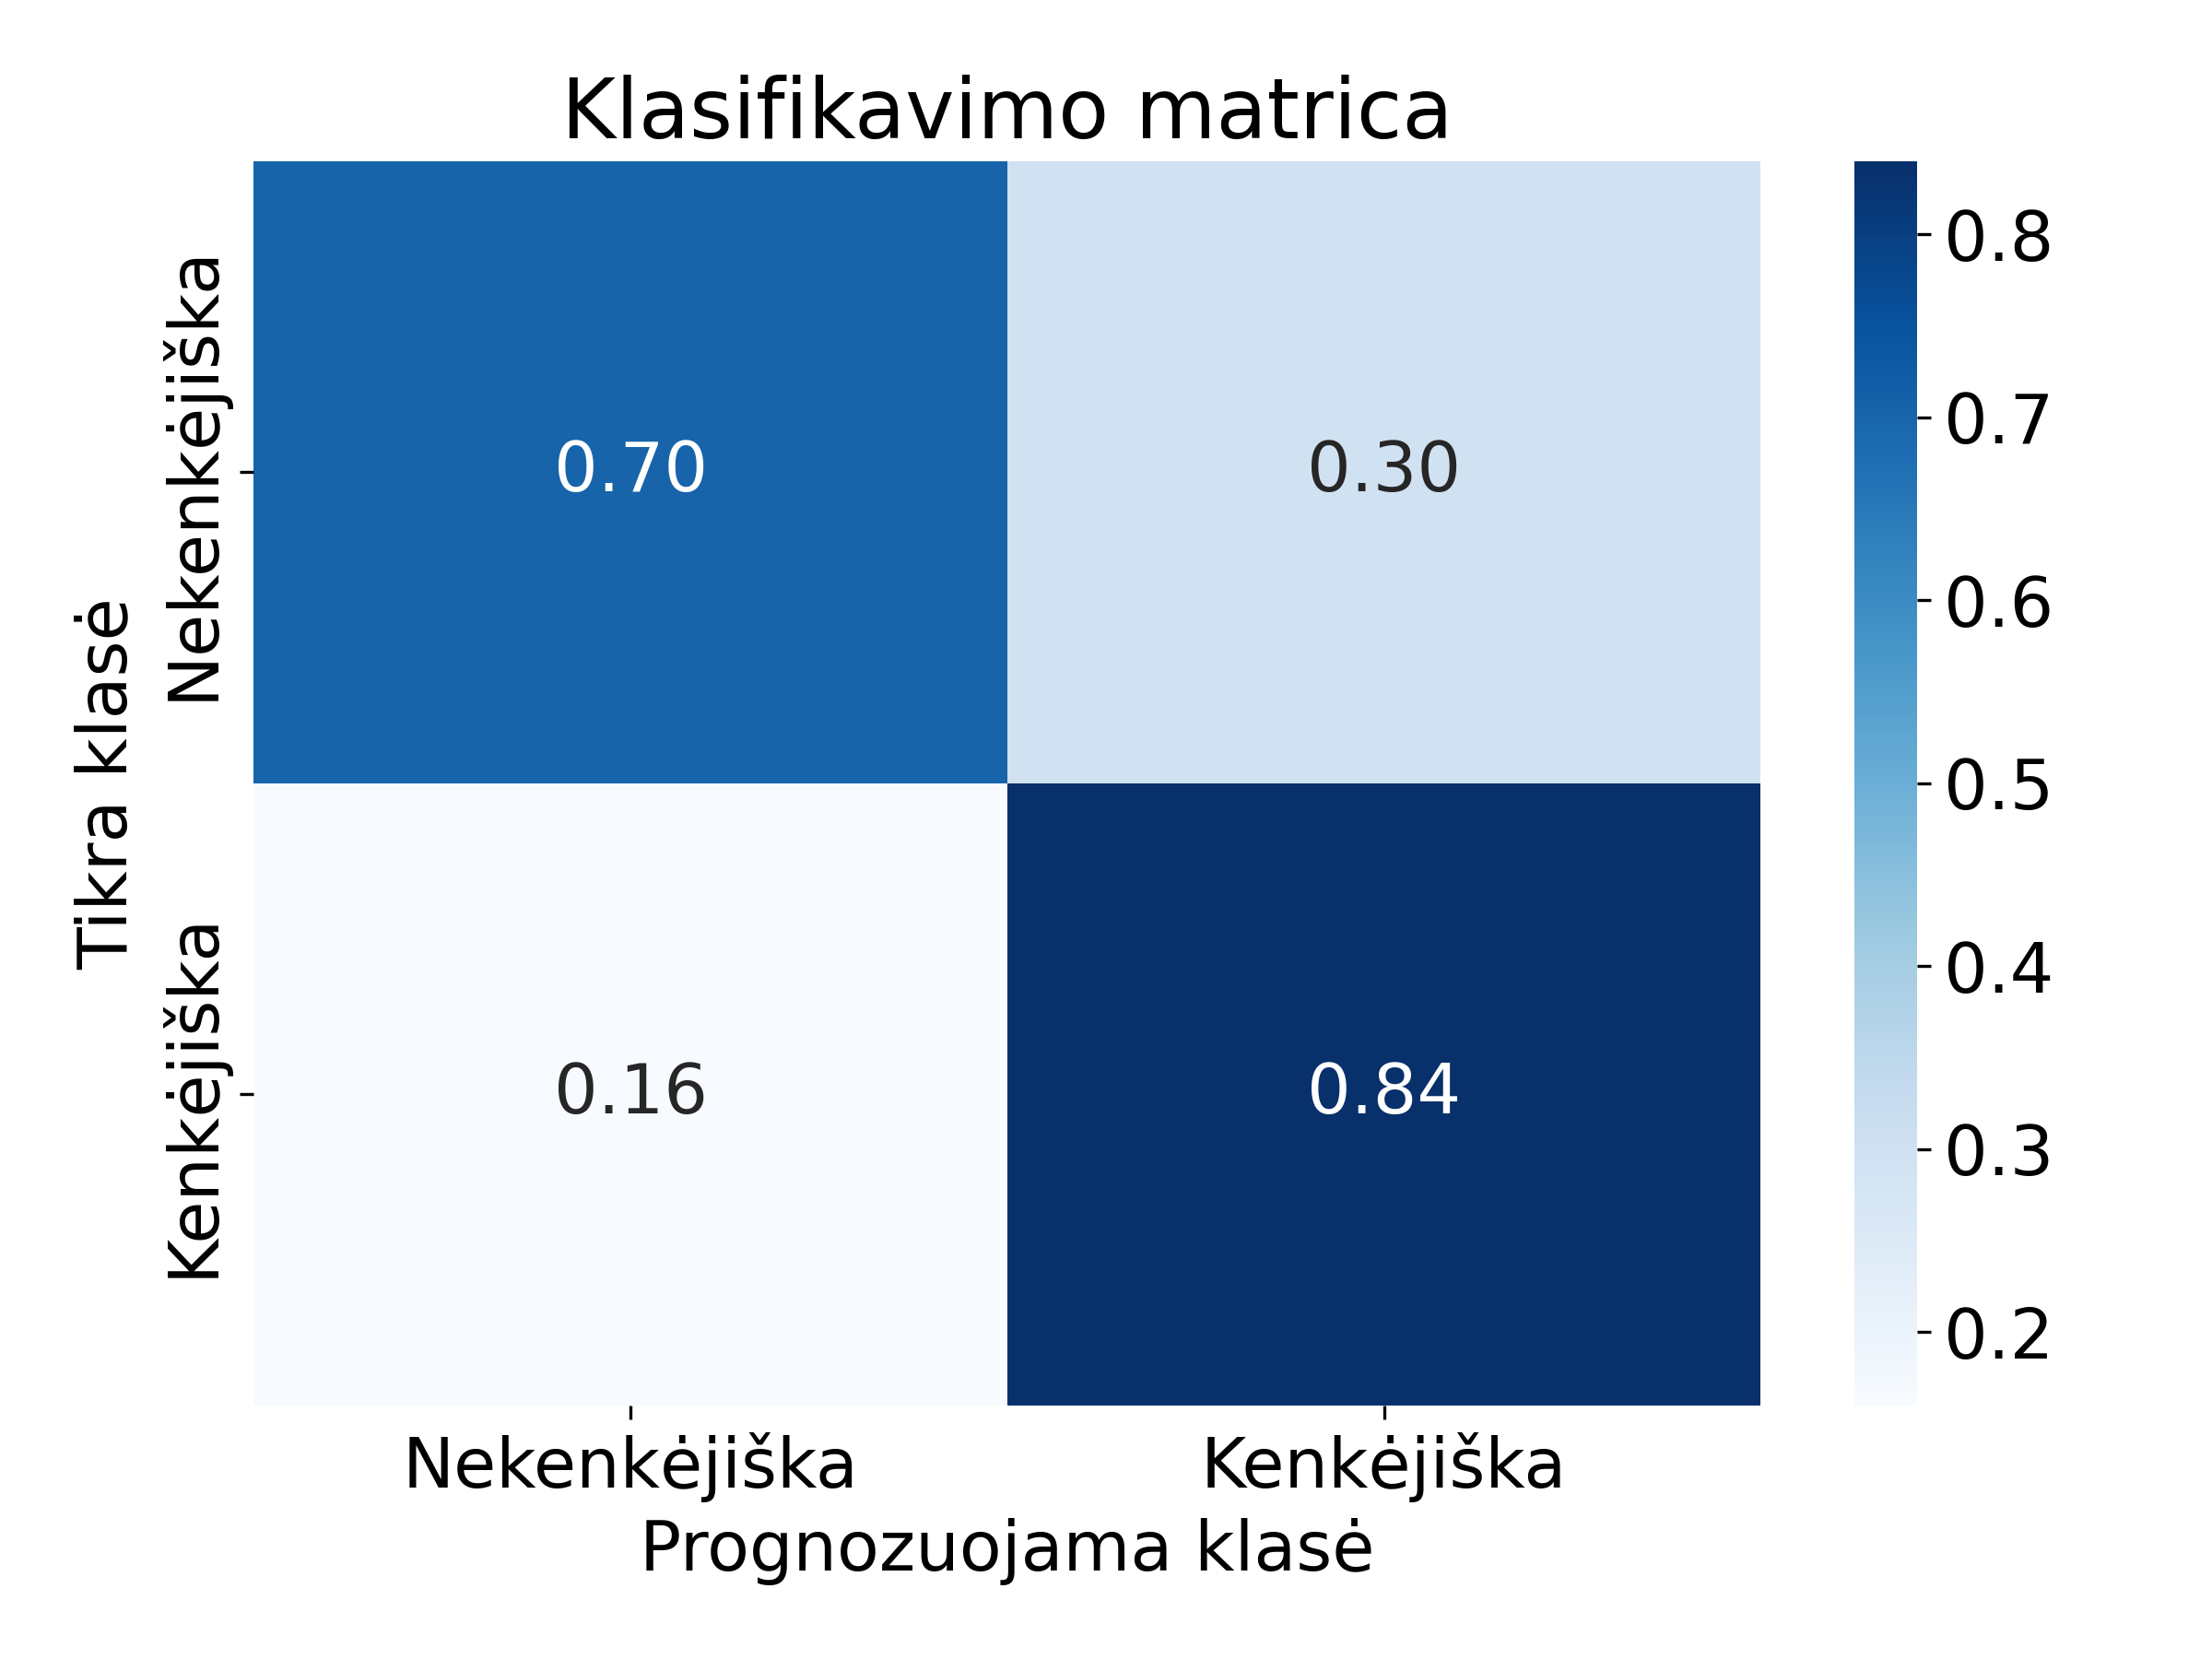
\includegraphics[width=\textwidth]{images/synthesis_2x2.png}
        \caption{Neišskiriant \textit{obfuskuotų} pavyzdžių klasės}
    \end{subfigure}
    \begin{subfigure}{0.5\textwidth}
        \centering
        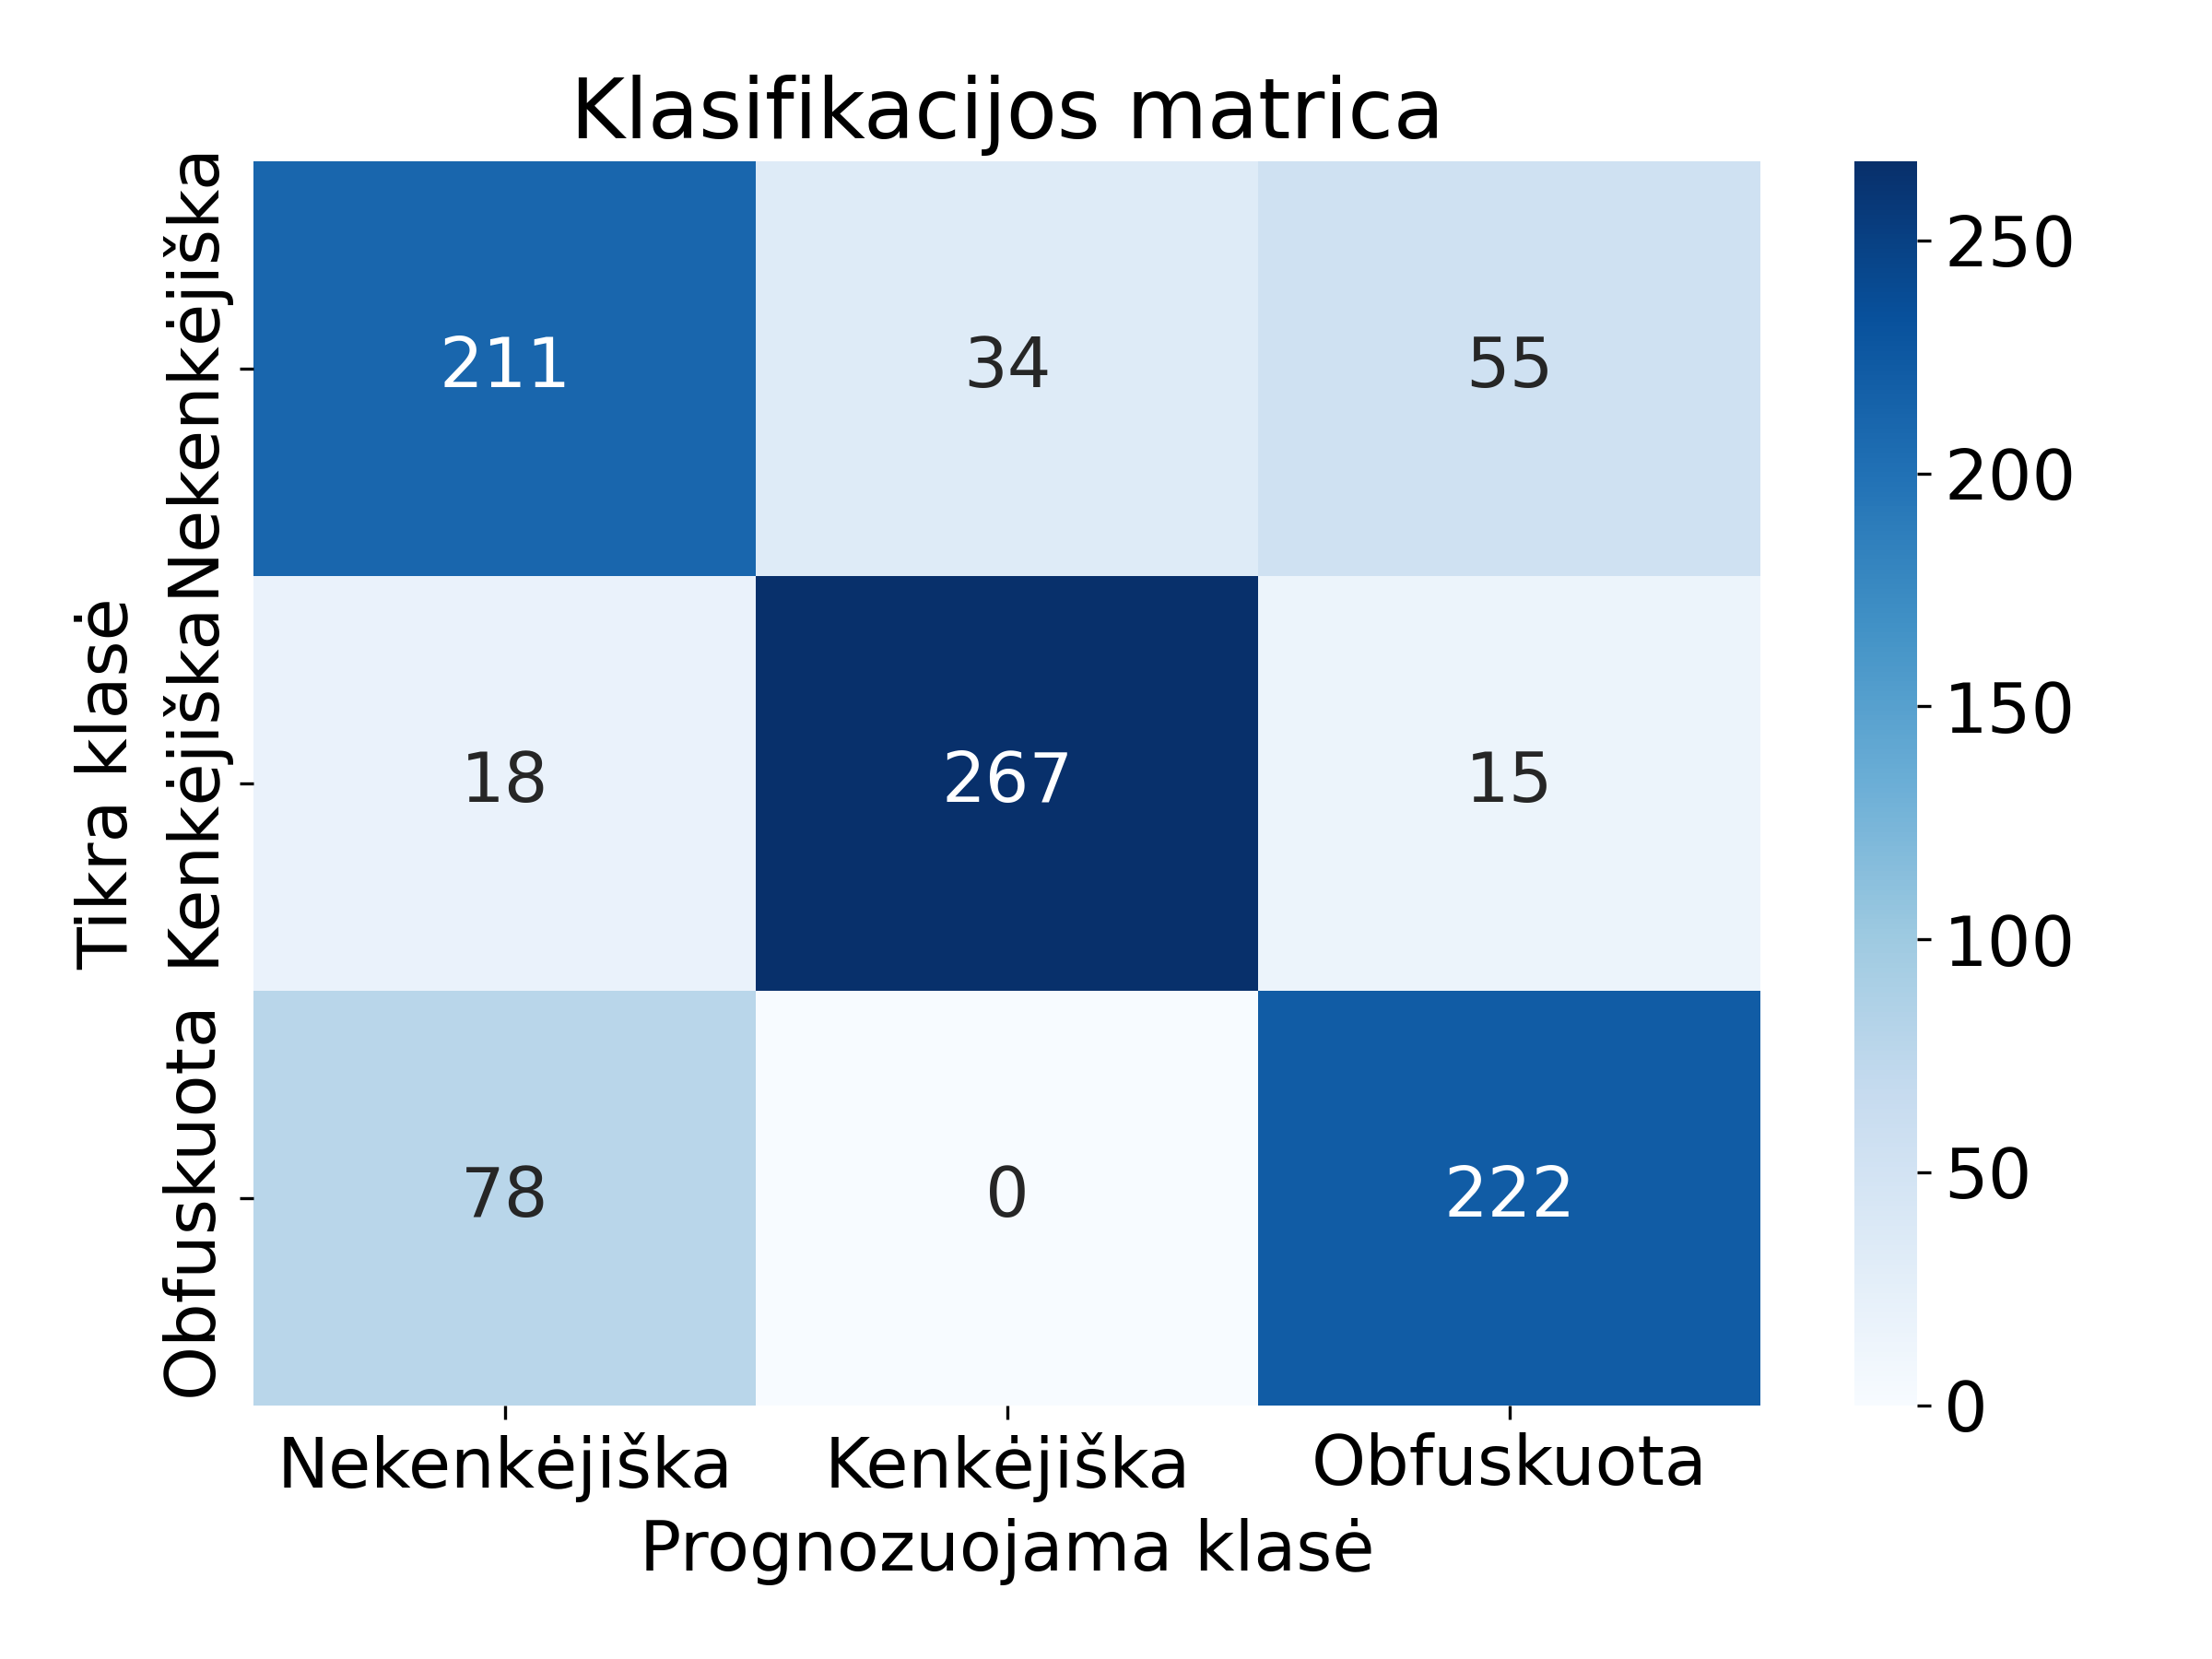
\includegraphics[width=\textwidth]{images/synthesis_3x3.png}
        \caption{Išskiriant \textit{obfuskuotų} pavyzdžių klasę}        
    \end{subfigure}
    \caption{\LIME ir \gls{mca} metodų sintezės klasifikavimo lentelės}
    \label{fig:exp3:confusion}
\end{figure}

\begin{table}[h]
    \caption{\LIME ir \gls{mca} metodų sintezės klasifikatoriaus metrikos (neišskiriant \textit{obfuskuotos} klasės)}
    \centering
    \exptable[\accLime]{tables/synthesis_2x2.csv}
    \label{tbl:exp3:metrics2}
\end{table}

\begin{table}[h]
    \caption{\LIME ir \gls{mca} metodų sintezės klasifikatoriaus metrikos (išskiriant \textit{obfuskuotą} klasę)}
    \centering
    \exptable[\accLimeObf]{tables/synthesis_3x3.csv}
    \label{tbl:exp3:metrics3}
\end{table}
